% --------------------------------------------------------------
% This is all preamble stuff that you don't have to worry about.
% Head down to where it says "Start here"
% --------------------------------------------------------------

\documentclass[12pt]{article}

\usepackage{fontspec}
\usepackage{xeCJK}
\usepackage[margin=1in]{geometry}
\usepackage{amsmath,amsthm,amssymb}
\usepackage{graphicx}

\setCJKmainfont{LiHei Pro}
\XeTeXlinebreaklocale zh
\XeTeXlinebreakskip = 0pt plus 1pt

% ------ Thm. Def. etc. ---------

% Theorem Styles
\newtheorem{theorem}{Theorem}[section]
\newtheorem{lemma}[theorem]{Lemma}
\newtheorem{proposition}[theorem]{Proposition}
\newtheorem{corollary}[theorem]{Corollary}
% Definition Styles
\theoremstyle{definition}
\newtheorem{definition}{Definition}[section]
\newtheorem{example}{Example}[section]
\theoremstyle{remark}
\newtheorem{remark}{Remark}

% ------ For pasting codes ------
\usepackage{listings}
\usepackage{color}

\definecolor{dkgreen}{rgb}{0,0.6,0}
\definecolor{gray}{rgb}{0.5,0.5,0.5}
\definecolor{mauve}{rgb}{0.58,0,0.82}

\lstset{frame=tb,
  language=C,
  aboveskip=3mm,
  belowskip=3mm,
  showstringspaces=false,
  columns=flexible,
  basicstyle={\small\ttfamily},
  numbers=none,
  numberstyle=\tiny\color{gray},
  keywordstyle=\color{blue},
  commentstyle=\color{dkgreen},
  stringstyle=\color{mauve},
  breaklines=true,
  breakatwhitespace=true,
  tabsize=3
}
% -----------------------------------

\begin{document}

% --------------------------------------------------------------
%                         Start here
% --------------------------------------------------------------

\title{Machine Learning Final Report}
\author{洪仲言 B00201015\\
蔡佳文 B00201025}
\maketitle
\section{Algorithm}
\subsection{Linear Model}
\begin{enumerate}
  \item {\em Logistic Regression\/}
  \item {\em Ridge Regression\/}
  \item {\em Linear SVM\/}
\end{enumerate}
\subsection{NonLinear Model}
\begin{enumerate}
  \item {\em SVM\/}
  \item {\em Random Forest\/}
\end{enumerate}
\section{Preprocess}
\subsection{Image}
\begin{enumerate}
  \item \large{\em \color{red}Resize\/}\\
    因為我們看見大家寫的字都東倒西歪的,如果直接將抓下來的資料拿來訓練一定很慘烈。\\
    所以我們用了兩種方式進行處理。
    \begin{enumerate}
      \item 將圖片用一個四邊形逼近,以減少太多空白的部分。只留下四邊形後,接著放大成122*105
      \item 將圖片用一個四邊形逼近,以減少太多空白的部分。把四邊形移到圖中心。為什麼會想這樣做呢?
        因為擔心放大後失去字的結構。可能『龍』這個字會因為放大,整團擠在一起。
    \end{enumerate}
  \item \large{\em \color{red}HOG\/}\\
    <<Histograms of Oriented Gradients for Human Detection>>是在2005年CVPR上發表的\\
    想用這個方法的原因是:就如同論文想要找到人在圖片裡麵和其他物體的互動(車子之類的),那他可是用梯度的方法找到
    人和車子。那我們是文字,我們拿到的資料裡面只有字還有一堆空白處,所以我們如果成順利找到字,並且將文字和空白分離
    這樣也許可以解決大家同樣的字在122*105裡面,出現在不同位子的情況。
  \item \large{\em \color{red}Scan Line\/}\\
    因為我們想處理的資料是中文字,如同大家所知道的,中文字是以字根或筆劃所構成,我們便嘗試以此為出發點之一。
    然而對字根的辨別太過困難,幾乎等同於對於較小的資料作中文字辨識,相當困難,故我們選用筆劃作為特徵。
    一個中文字的筆劃有許多方向,且多是接近直線,如「大」字就有三個方向的略為彎曲筆劃。我們就以圖中出現的各個方向的直線線段作為特徵。
    例如 $L = \text{圖片} \cup \text{某直線線段}$, 則基於此直線線段的特徵為$f(L) = \frac{\sqrt{\sum len(l_i)^2}}{len(L)}$, 其中 $l_i$ 為直線線段上的連續白色子線段(即有與字重疊的部份)。
    我們希望能透過筆劃與筆劃之間的關聯,使的機器學習到「字」的樣子,進而在結果上有好的表現。
\end{enumerate}
\subsection{Class}
\begin{enumerate}
  \item \large{\em \color{red}合併\/}\\
  因為在track0上面,『一』判斷成『壹』也算是得分,反之亦然。所以我想說可不可以在class上面降維,把所有class > 21的
    都減掉10。但是結果似乎不太理想,可能令model感到疑惑了。
\end{enumerate}
\section{Bagging and Blending}
\subsection{Bagging}
\begin{enumerate}
  \item 對linear svm 進行Bagging 100 參數C: 1 \\
    效果不錯 0.28 $ \to $ 0.267
  \item 對kernel svm 進行Bagging 100  參數$ \text{kernel: rbf, C: 100,} \gamma \text{: 0.1} $\\
    實驗進行到一半\dots\dots 收到網管的信memory leaks QQ ,雖然比賽很重要
    ,但是跟實驗室學長姐的感情也很重要所以忍痛放棄這個實驗。
  \item 對ramdom forest 進行 Bagging 100 參數 870顆樹\\
    Random Forest 本身就是一個Bagging的演算法了,想說試試看會不會發生什麼怪異的事情,但是
    跑了好久還沒跑完,所以在四天後放棄這個探險。
  \item 對LogisticRegression 和 RidgeRegression 進行Bagging 100 參數各為c=10 $ \alpha = 10$
\end{enumerate}
\subsection{Blending}
\begin{enumerate}
  \item 對進行公平投票的方法,看哪個過半數,如果都沒有的話,隨機選一個答案\\
    <{\em SVM:\/} kernel=rbf C=125 $ \gamma = 0.12 $>\\ 
    <{\em Random Forest:\/} tree=870 max\_feature=sqrt> \\
    <{\em SVM linear:\/} c=1 bagging=100>\\
    成果有進步 0.24 (三個臭皮匠勝過一個臭皮匠)
  \item 對進行公平投票的方法,看哪個過半數,如果都沒有的話,選一個較多的,如果有一樣票數最多的,在隨機選一個\\
    <{\em SVM:\/} kernel=rbf C=125 $ \gamma = 0.12 $>\\ 
    <{\em Random Forest:\/} tree=870 max\_feature=sqrt> \\
    <{\em SVM linear:\/} c=1 bagging=100>\\
    <{\em Logistic regression:\/} c=1>\\
    <{\em Ridge regression:\/} c=10>\\
    成果有進步 0.25 但是相較於上一個Blending竟然退步了,可能是因為人多口雜,好的事情被淹沒了
  \item 對進行公平投票的方法,看哪個過半數,如果都沒有的話,選一個較多的,如果有一樣票數最多的,在隨機選一個\\
    <{\em SVM:\/} kernel=rbf C=125 $ \gamma = 0.12 $>\\ 
    <{\em SVM:\/} kernel=rbf C=100 $ \gamma = 0.12 $>\\ 
    <{\em Random Forest:\/} tree=870 max\_feature=sqrt> \\
    <{\em SVM linear:\/} c=1 bagging=100>\\
    <{\em SVM linear:\/} c=1 >\\
    <{\em Logistic regression:\/} c=1>\\
    <{\em Ridge regression:\/} c=10>\\
    成果沒進步 0.29 但是相較於上一個Blending竟然退步了,果然太多臭皮匠會讓事情變糟
\end{enumerate}
\section{Best Result}
經過一連串的時候發現還是原始的資料搭配使用HOG的效果最好。
反而我自己Resize後在使用HOG的效果沒那麼好,可能是因為我的Resize用壞原本的資料形狀了。\\
而在原始資料上做Random Forest是表現最好的,不做HOG時可以到0.65其他演算法都在0.7~0.8遊蕩。
Overfitting非常嚴重,我認為是因為在為處理的data非常雜亂。光看『一』這個字:\\
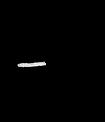
\includegraphics[width=1.5cm, height=1.5cm]{./photo44.jpg}一個寫在正中間\\
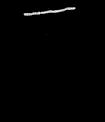
\includegraphics[width=1.5cm, height=1.5cm]{./photo228.jpg}一個寫到天上去了\\
這樣會讓演算法學不好,因為對他們來說一個像素是一個feature所以如果演算法學到在100到110之間有值是『一』。那寫在不同位子的『一』可能會讓演算法誤判\\
但是一做HOG之後,都用向量表示,這樣子雜訊就變少,而SVM展現自己的價值,馬上變成最強的演算法了。\\
而 Scan Line 的部份,則因負責生的人寫的太慢了,導致能用來測試的時間很少。
不過在結果上大多是贏過hog的,或許是因為他的feature是特別對文字產生的?hog有些特性在文字上比較無法體現,像是對圖片處理顏色、光影變化等,在文字中就會無法使用。\\
目前 SVM 與 Scan Line 最匹配,效果最好,與 hog 類似。不過他跟 random forest 就相當不合拍,其 $E_out$ 也大幅度的超越了 logistic regression 。\\
或許我們可以稱為「不同的 feature 對不同的 learner 適應性可能有顯著差異」。
\subsection{For each algorithm with HOG}
\scalebox{0.8}{
\begin{tabular}{|l|l|l|l|l|l|l|}
\hline
\textbf{algorithm/with hog}                                                  & \textbf{c}   & \textbf{gamma} & \textbf{kernel} & \textbf{bagging} & \textbf{tree} & \textbf{e\_out} \\ \hline
\textbf{SVM}                                                                 & \textbf{100} & \textbf{0.12}  & \textbf{rbf}    & \textbf{}        & \textbf{}     & \textbf{0.26}  \\ \hline
\textbf{SVM}                                                                 & \textbf{125} & \textbf{0.12}  & \textbf{rbf}    & \textbf{}        & \textbf{}     & \textbf{0.26}  \\ \hline
\textbf{LinearSVM}                                                           & \textbf{10}  & \textbf{}      & \textbf{}       & \textbf{}        & \textbf{}     & \textbf{0.28}  \\ \hline
\textbf{LinearSVM}                                                           & \textbf{10}  & \textbf{}      & \textbf{}       & \textbf{100}     & \textbf{}     & \textbf{0.27}   \\ \hline
\textbf{LogisticRegression}                                                  & \textbf{10}  & \textbf{}      & \textbf{}       & \textbf{}        & \textbf{}     & \textbf{0.32}   \\ \hline
\textbf{LogisticRegression}                                                  & \textbf{10}  & \textbf{}      & \textbf{}       & \textbf{100}        & \textbf{}     & \textbf{0.29}   \\ \hline
\textbf{RidgeRegression}                                                     & \textbf{alpha=10}    & \textbf{}      & \textbf{}       & \textbf{}        & \textbf{}     & \textbf{0.44}       \\ \hline
\textbf{RidgeRegression}                                                     & \textbf{alpha=10}    & \textbf{}      & \textbf{}       & \textbf{100}        & \textbf{}     & \textbf{0.38}       \\ \hline
\textbf{RandomForest}                                                        & \textbf{}    & \textbf{}      & \textbf{}       & \textbf{}        & \textbf{870}  & \textbf{0.28}   \\ \hline
\end{tabular}
}

\subsection{For Scan Line}
\scalebox{0.8}{
\begin{tabular}{|l|l|l|l|l|}
\hline
\textbf{algorithm/with scan line} & \textbf{c} & \textbf{gamma} & \textbf{tree} & \textbf{e\_out} \\ \hline
\textbf{SVM}                      & \textbf{8} & \textbf{0.007} &               & \textbf{0.187}  \\ \hline
\textbf{RandomForest}             &            &                & \textbf{870}  & \textbf{0.27}   \\ \hline
\textbf{LogisticRegression}             &  \textbf{10}          &                &   & \textbf{0.215}   \\ \hline
\end{tabular}}

\subsection{For each blending}
\scalebox{0.8}{
\begin{tabular}{|l|l|}
\hline
\textbf{Blending}                                                                                                   & \textbf{e\_out} \\ \hline
\textbf{RF+SVM\_c=125+LinearSVM}                                                                                           & \textbf{0.24}   \\ \hline
\textbf{RF+SVM\_c=125+LinearSVM+LogisticReg+RidgeReg}                                                                      & \textbf{0.25}   \\ \hline
\textbf{\begin{tabular}[c]{@{}l@{}}RF+SVM\_c=100+SVM\_c=125+LinearSVM+LinearSVM\_bag\\ +LogisticReg+RidgeReg\end{tabular}} & \textbf{0.29}   \\ \hline
\end{tabular}}

\subsection{Best Approach}
So for both of track0 and track1: the best approach is {\color{red}Blending: SVM + RandomForest + LinearSVM}\\
這個Blending方法的優缺點(我相信如果是搭配Scan Line的feature應該效果會更好。目前的實驗結果是搭配HOG的)
\begin{enumerate}
    \item 優點:使用Blending的方法,可以達到三個臭皮匠勝過一個諸葛亮的境界,因為各自的演算法有他自己的盲點,多一點不一樣的意見可能會讓演算法表現得更好。對於最佳的演算法(SVM) 進行每一筆的預測:錯誤的地方也許會被其他演算法給糾正,而如果是對的地方那其他演算法也能如願支持的話那更容易是對的,所以這個Blending的方法是會讓成果更進步的。
    \item 缺點:就是你必須先Train出三個Model,這將會耗掉非常多的時間。而且公平投票這個方法是否真的是正確的呢?是不是比較強大的Model應該要有比較大的分數呢?難道多數就是對的?也許有方法可以調出更好的權重,票票等值也許是有問題的。
\end{enumerate}

\section{工作分配}
\begin{enumerate}
    \item 洪仲言:HOG, Bagging, Blending, Random Forest, SVM, LinearSVM\\
    \item 蔡佳文:Scan Line, Resize, LogisticRegression, RidgeRegression
\end{enumerate}
\end{document}
